% Graphic for TeX using PGF
% Title: /home/marta/Diagrama2.dia
% Creator: Dia v0.97.3
% CreationDate: Sat Sep  9 00:01:27 2017
% For: marta
% \usepackage{tikz}
% The following commands are not supported in PSTricks at present
% We define them conditionally, so when they are implemented,
% this pgf file will use them.
\ifx\du\undefined
  \newlength{\du}
\fi
\setlength{\du}{15\unitlength}
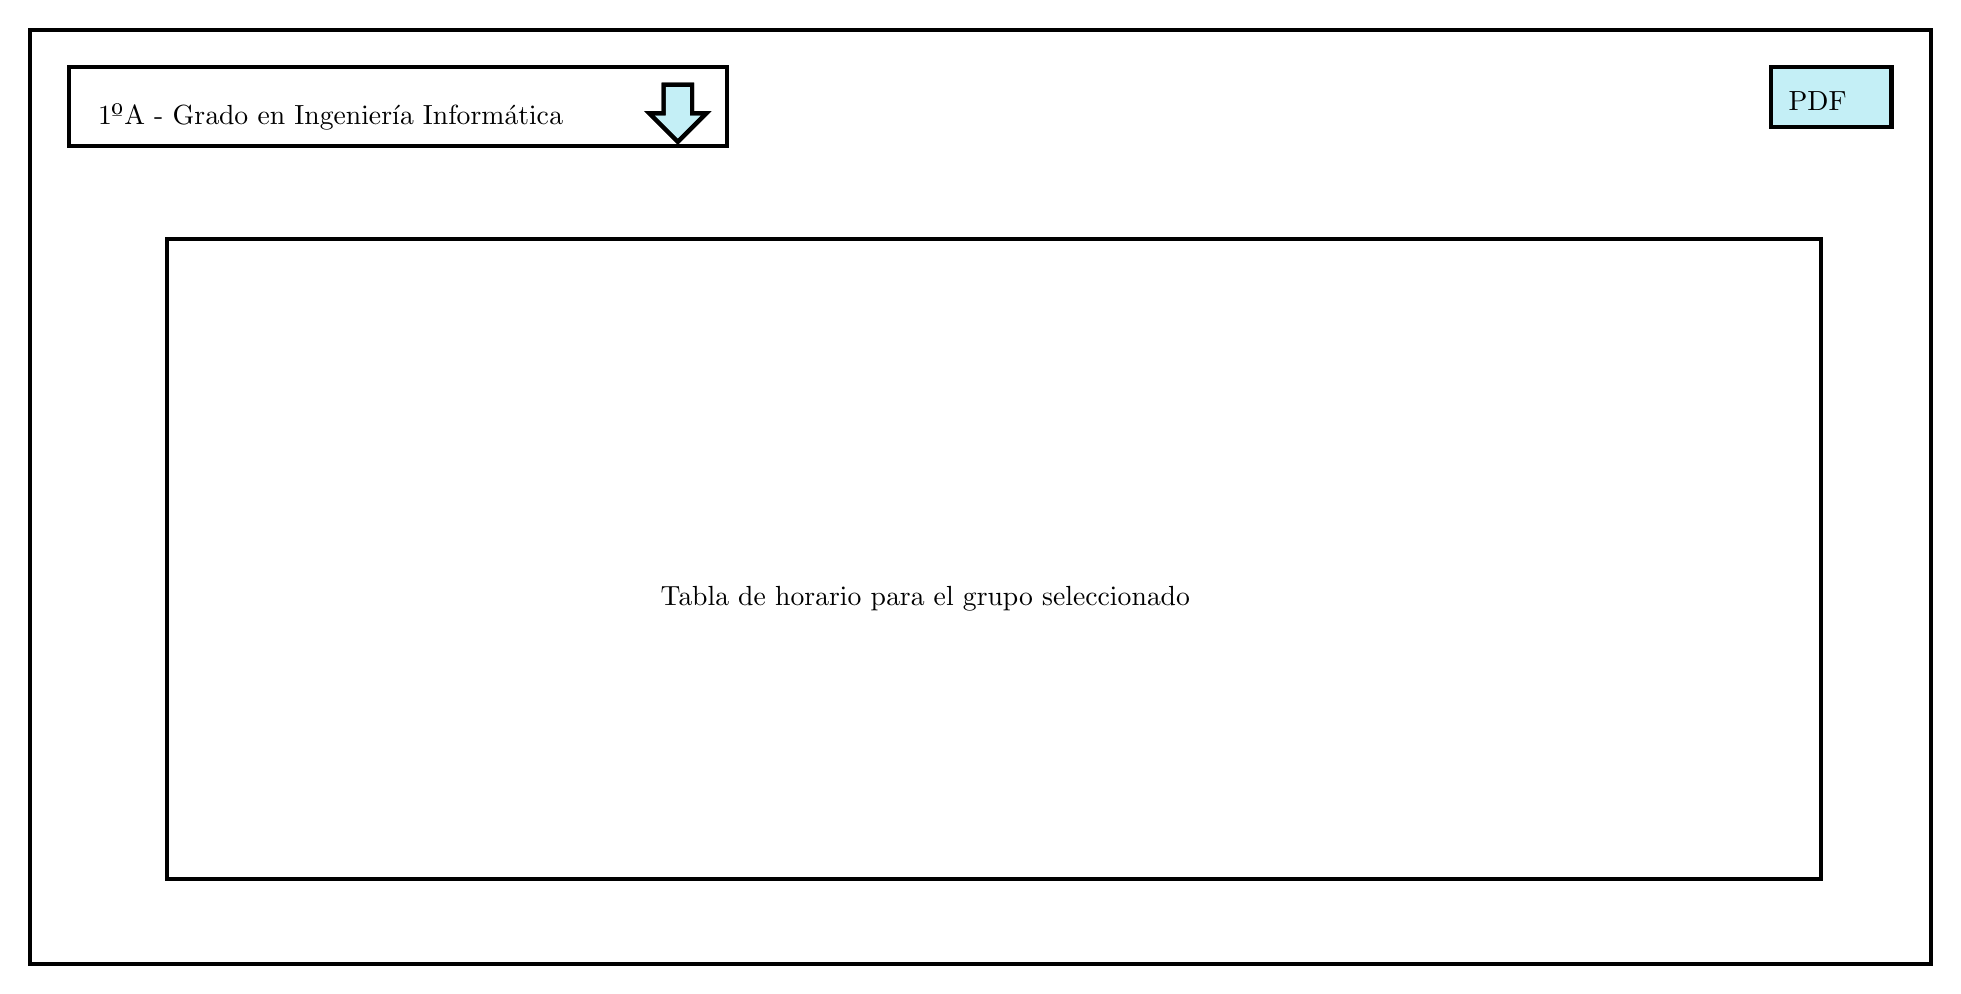
\begin{tikzpicture}
\pgftransformxscale{1.000000}
\pgftransformyscale{-1.000000}
\definecolor{dialinecolor}{rgb}{0.000000, 0.000000, 0.000000}
\pgfsetstrokecolor{dialinecolor}
\definecolor{dialinecolor}{rgb}{1.000000, 1.000000, 1.000000}
\pgfsetfillcolor{dialinecolor}
\pgfsetlinewidth{0.100000\du}
\pgfsetdash{}{0pt}
\pgfsetdash{}{0pt}
\pgfsetmiterjoin
\definecolor{dialinecolor}{rgb}{1.000000, 1.000000, 1.000000}
\pgfsetfillcolor{dialinecolor}
\fill (4.900000\du,2.550000\du)--(4.900000\du,25.050000\du)--(50.700000\du,25.050000\du)--(50.700000\du,2.550000\du)--cycle;
\definecolor{dialinecolor}{rgb}{0.000000, 0.000000, 0.000000}
\pgfsetstrokecolor{dialinecolor}
\draw (4.900000\du,2.550000\du)--(4.900000\du,25.050000\du)--(50.700000\du,25.050000\du)--(50.700000\du,2.550000\du)--cycle;
\pgfsetlinewidth{0.100000\du}
\pgfsetdash{}{0pt}
\pgfsetdash{}{0pt}
\pgfsetmiterjoin
\definecolor{dialinecolor}{rgb}{1.000000, 1.000000, 1.000000}
\pgfsetfillcolor{dialinecolor}
\fill (5.850000\du,3.450000\du)--(5.850000\du,5.350000\du)--(21.700000\du,5.350000\du)--(21.700000\du,3.450000\du)--cycle;
\definecolor{dialinecolor}{rgb}{0.000000, 0.000000, 0.000000}
\pgfsetstrokecolor{dialinecolor}
\draw (5.850000\du,3.450000\du)--(5.850000\du,5.350000\du)--(21.700000\du,5.350000\du)--(21.700000\du,3.450000\du)--cycle;
\pgfsetlinewidth{0.100000\du}
\pgfsetdash{}{0pt}
\pgfsetdash{}{0pt}
\pgfsetbuttcap
\pgfsetmiterjoin
\pgfsetlinewidth{0.100000\du}
\pgfsetbuttcap
\pgfsetmiterjoin
\pgfsetdash{}{0pt}
\definecolor{dialinecolor}{rgb}{0.768627, 0.937255, 0.964706}
\pgfsetfillcolor{dialinecolor}
\fill (20.168750\du,3.875000\du)--(20.168750\du,4.562500\du)--(19.825000\du,4.562500\du)--(20.512500\du,5.250000\du)--(21.200000\du,4.562500\du)--(20.856250\du,4.562500\du)--(20.856250\du,3.875000\du)--cycle;
\definecolor{dialinecolor}{rgb}{0.000000, 0.000000, 0.000000}
\pgfsetstrokecolor{dialinecolor}
\draw (20.168750\du,3.875000\du)--(20.168750\du,4.562500\du)--(19.825000\du,4.562500\du)--(20.512500\du,5.250000\du)--(21.200000\du,4.562500\du)--(20.856250\du,4.562500\du)--(20.856250\du,3.875000\du)--cycle;
\pgfsetbuttcap
\pgfsetmiterjoin
\pgfsetdash{}{0pt}
\definecolor{dialinecolor}{rgb}{0.000000, 0.000000, 0.000000}
\pgfsetstrokecolor{dialinecolor}
\draw (20.168750\du,3.875000\du)--(20.168750\du,4.562500\du)--(19.825000\du,4.562500\du)--(20.512500\du,5.250000\du)--(21.200000\du,4.562500\du)--(20.856250\du,4.562500\du)--(20.856250\du,3.875000\du)--cycle;
% setfont left to latex
\definecolor{dialinecolor}{rgb}{0.000000, 0.000000, 0.000000}
\pgfsetstrokecolor{dialinecolor}
\node[anchor=west] at (6.275000\du,4.650000\du){1ºA - Grado en Ingeniería Informática};
\pgfsetlinewidth{0.100000\du}
\pgfsetdash{}{0pt}
\pgfsetdash{}{0pt}
\pgfsetmiterjoin
\definecolor{dialinecolor}{rgb}{0.768627, 0.937255, 0.964706}
\pgfsetfillcolor{dialinecolor}
\fill (46.850000\du,3.450000\du)--(46.850000\du,4.900000\du)--(49.750000\du,4.900000\du)--(49.750000\du,3.450000\du)--cycle;
\definecolor{dialinecolor}{rgb}{0.000000, 0.000000, 0.000000}
\pgfsetstrokecolor{dialinecolor}
\draw (46.850000\du,3.450000\du)--(46.850000\du,4.900000\du)--(49.750000\du,4.900000\du)--(49.750000\du,3.450000\du)--cycle;
% setfont left to latex
\definecolor{dialinecolor}{rgb}{0.000000, 0.000000, 0.000000}
\pgfsetstrokecolor{dialinecolor}
\node[anchor=west] at (47.000000\du,4.275000\du){PDF};
\pgfsetlinewidth{0.100000\du}
\pgfsetdash{}{0pt}
\pgfsetdash{}{0pt}
\pgfsetmiterjoin
\definecolor{dialinecolor}{rgb}{1.000000, 1.000000, 1.000000}
\pgfsetfillcolor{dialinecolor}
\fill (8.200000\du,7.600000\du)--(8.200000\du,23.000000\du)--(48.050000\du,23.000000\du)--(48.050000\du,7.600000\du)--cycle;
\definecolor{dialinecolor}{rgb}{0.000000, 0.000000, 0.000000}
\pgfsetstrokecolor{dialinecolor}
\draw (8.200000\du,7.600000\du)--(8.200000\du,23.000000\du)--(48.050000\du,23.000000\du)--(48.050000\du,7.600000\du)--cycle;
% setfont left to latex
\definecolor{dialinecolor}{rgb}{0.000000, 0.000000, 0.000000}
\pgfsetstrokecolor{dialinecolor}
\node[anchor=west] at (19.825000\du,16.250000\du){Tabla de horario para el grupo seleccionado};
\end{tikzpicture}
